
%%
%%  Beam Loading Paper '17
%% ***************************
%%  Veronica K. Berglyd Olsen
%%

\documentclass[aps,prstab,reprint,amsmath,amssymb,groupedaddress]{revtex4-1}
\bibliographystyle{apsrev4-1}

\usepackage{hyperref}
\hypersetup{colorlinks=true, citecolor=blue, urlcolor=blue, linkcolor=blue}

\usepackage{graphicx}


% Custom Commands
%*****************

% Text
%~ \newcommand{\eq}[1]{Eq. \ref{#1}}
%~ \newcommand{\fig}[1]{Fig. \ref{#1}}
%~ \newcommand{\tbl}[1]{Table \ref{#1}}

% Math
\newcommand{\unit}[1]{\,\mathrm{#1}}
\newcommand{\funit}[2]{\,\mathrm{#1}/\mathrm{#2}}
\newcommand{\mexp}[1]{\mathrm{e}^{#1}}
\newcommand{\nexp}[1]{\times 10^{#1}}

% ******************************************************************************************************************** %
\begin{document}
% ******************************************************************************************************************** %

%~ Eric's Comments
%~ Sec N: Beam loading [in this section we describe the interesting physics, based on a single parameters set]
%~ - describe proton beam wake structure [similar to that of a modulated proton beam] (simulation results to show:
%~   unloaded wake)
%~ - by varying the current of the electron beam, the electron beam may load the wake and the longitudinal field can be
%~   flatten and energy spread reduced [well known result, Tzoufras] 
%~ - the electron beam blows out the remaining plasma electrons. The transverse fields are dominated by the linear
%~   focusing fields originating from the ion background, leading to emittance preservation of the part of the electron
%~   beam inside the bubble [loading of a quasi-linear wake, and still get emittance preservation: this is new]
%~   (simulation results to show: loaded wake, with bubble - many different aspects of this, trans., long. field,
%~   electron densities etc. )
%~ - the acceleration and the transverse emittance stable on long timescales (simulation results to show: transverse and
%~   longitudinal phase spaces, space long simulation)
%~ - in this regime, emittance preservation is robustness to drive-witness offset [this is new] (simulation results to
%~   show: transverse and longitudinal phase spaces, long offset simulation)
%~ Sec N+1: Parameter optimization, or, parameter scaling [in this section we describe how to optimize the electron
%~ beam, and preferably some scalings]
%~ - how to select electron beam parameters:
%~ - longitudinal parameters bunch length and current (simulations results to show: overloaded/underloaded cases)
%~ - transverse parameters of electron emittance / matching [too large, outside bubble.  Do we see increased head
%~   erosion -> faster decay]?  (simulations results to show: evolution of high emittance vs low emittance cases)
%~ (- plasma density?)


%~ Patric's Comments
%~ - Self-modulation as a driver
%~ - SM does not reach blow out
%~ - SM does not preserve emittance and produces large energy spread and parameters may evolve along the accelerator,
%~   not desirable
%~ - Beam loading for narrow energy spread
%~ - Beam loading in linear regime (old papers from SLAC in the 80's, then Katsouleas for PWFA) and nonlinear regime
%~   (Tzoufras) well know
%~ - Propose "new regime" in the SM case, beam loading and blowout to get emittance preservation
%~ - Limitation as for PWFA driver, must use some of the W bunch to reach the blowout, it is kind of like the early SLAC
%~   experiments (84GeV) where the W-bunch is like the D-bunch in these experiments, but in a plasma prepared by the p+
%~   bunch and the SM
%~ - maybe also something about the fact that 200pC in a 60µm bunch corresponds to a 1kA current, much larger than the
%~   p+ bunch current, because of the fact that the wakefields are driven my multiple bunches?
%~ As for N+2, I am a firm supporter of on-axis injection ... and most of the issue with that has to do with the plasma
%~ ramp, otherwise it would be a non-issue (assuming of course that one can split the plasma in two sections). It is in
%~ itself a topic of research, so I think we can only state a few things ...


\title{Emittance preservation of an electron bunch in a loaded quasi-linear plasma wakefield}

\author{Veronica K. Berglyd Olsen}
\email[]{v.k.b.olsen@cern.ch}

\author{Erik Adli}
\affiliation{University of Oslo, Oslo, Norway}

\author{Patric Muggli}
\affiliation{Max Planck Institute for Physics, Munich, Germany}
\affiliation{CERN, Geneva, Switzerland}

\date{\today}

\begin{abstract}
We investigate beam loading and emittance preservation for a high-charge electron beam being accelerated in quasi-linear
plasma wakefield driven by a short proton beam. The structure of the wakefield is similar to that of a long, modulated
proton beam. By selecting transverse and longitudinal electron beam parameters in order to appropriately load the wake,
we show that the bulk of the electron beam can be accelerated without significant emittance growth.
\end{abstract}

\maketitle

% ******************************************************************************************************************** %
\section[\label{S:I}]{Introduction}
% interested from SMI/AWAKE
% requirements for AWAKE Run 2
% ******************************************************************************************************************** %

Beam driven plasma wakefield accelerators have the potential to offer compact linear accelerators with high energy
gradients, and has been of interest for several decades \cite{chen:1985}. A relativist beam travelling through a plasma
will excite a strong longitudinal e-field that can be loaded by a trailing witness beam, which can achieve a high
acceleration gradient. Acceleration of an electron beam by an electron drive bunch has been demonstrated experimentally
\cite{rosenzweig:1988, blumenfeld:2007, kallos:2008} in the past. The AWAKE experiment at CERN is a proof of concept
proton driven plasma wakefield accelerator \cite{awake_collaboration:2014}.

A major challenge with plasma wakefield accelerators is, however, to produce an accelerated beam with a minimal increase
in energy spread and emittance. In the well described linear case where the beam density $n_{b}$ is much smaller than
the plasma density $n_{0}$ the plasma causes emittance growth in the beam. A finite length beam will also see a varying
transverse wakefield causing increasing energy spread \cite{katsouleas:1987}. In the non-linear regime, where
$n_{b} > n_{0}$, the drive beam sees an unvarying transverse field due to a bubble forming in the plasma behind the
drive beam. The bubble is formed by the transverse oscillations of the plasma electrons which move near uniformly as a
function of distance from the drive beam forming a sheet around an evacuated area. Since the much heavier plasma ions
have no significant movement within the relevant time frame, these remaining ion channel creates a focusing force that
scales linearly with the radius within this bubble producing a angularly symmetric focusing force
\cite{lu:2006-1, lu:2006}. This effect also avoid the issue of increasing energy spread due to transverse beam loading.
Increase in energy spread is still dependent on beam loading of the longitudinal e-field, $E_{z}$. This effect can be
negated by specially shaped beams \cite{katsouleas:1987, tzoufras:2009}, but this is difficult experimentally and is not
a topic explored in this paper.

% ******************************************************************************************************************** %
\subsection[\label{S:I:SMI}]{Self-modulation as a Driver}
%~ Patric's Comments
%~ - Self-modulation as a driver
%~ - SM does not reach blow out
%~ - SM does not preserve emittance and produces large energy spread and parameters may evolve along the accelerator,
%~   not desirable
% ******************************************************************************************************************** %

A train of electron drive bunches with a separation $\lambda_{pe}$ and a length $l_{b} \ll \lambda_{pe}$, where
$\lambda_{p} = 2\pi c/\omega_{pe}$ and $\omega_{pe} = (n_{0} e^{2} / m_{e} \epsilon_{0})^{1/2}$, will drive an
increasingly strong field $E_{z}$ for each bunch \cite{chen:1985}. A tailing witness beam loading the peak accelerating
phase of this field will quickly gain energy from the wakefield. Acceleration of an electron witness beam driven by two
electron drive beams was demonstrated at Brookhaven National Laboratory \cite{muggli:2011}. However, electron drive
bunches will quickly lose energy to the plasma, and the accelerating witness beam will eventually catch up with the
drive beam and the acceleration stop.

This de-phasing problem can be minimised by instead using a proton drive bunch \cite{caldwell:2009}. Proton beams, like
for instance the LHC and SPS beams at CERN, are ideal candidates for such an accelerator; however, they are orders of
magnitude longer than the plasma wavelengths needed for such applications. This issue is resolved by letting the proton
beam undergo self-modulation before injecting the witness beam into one of the buckets in the modulated structure. This
self-modulation instability is caused by the transverse fields generated by the beam acting upon the beam itself,
causing regions of the beam to rapidly defocus \cite{kumar:2010}. The modulation frequency is close to that of the
plasma, leaving a train of proton bunches along the beam axis.

% ******************************************************************************************************************** %
\subsection[\label{S:I:AWAKE}]{The AWAKE Experiment}
% ******************************************************************************************************************** %

The AWAKE experiment, currently in its first stages of operation at CERN, uses the SPS beam as its driver. The first run
of the experiment is set up with a $10\unit{m}$ rubidium plasma cell, with a nominal plasma density of
$7\nexp{14}\unit{cm}^{-3}$ \cite{gschwendtner:2016}. The corresponding plasma wavelength is $1.26\unit{mm}$. The plasma
density is matched to the SPS proton beam such that $k_{pe}\sigma_{r} = 1$ where $k_{pe} = \lambda_{pe}/2\pi$ is the
plasma wave number. The aim of the first run is to demonstrate self-modulation of the proton beam, and in 2018 to
sample the wake field with a long electron bunch. The study presented here is for run two, which aims to demonstrate
acceleration of a short electron bunch producing at high energy and low emittance and low energy spread.

\begin{figure}[hbt]
    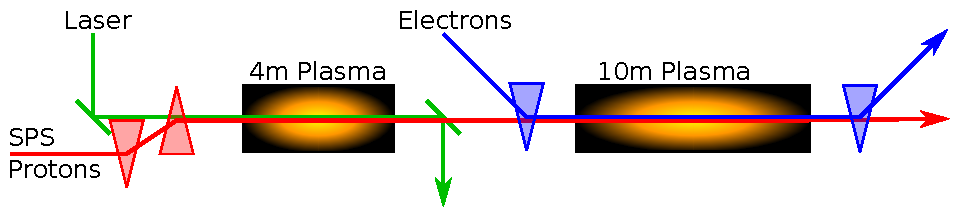
\includegraphics[width=0.99\linewidth,trim={1mm 2mm 1mm 2mm},clip]{figures/figAWAKE}
    \caption{\label{Fig:AWAKER2} A simplified illustration of the experimental setup for AWAKE Run 2. The SPS proton
        beam undergoes self-modulation in the first $4\unit{m}$ plasma cell. The electron witness beam is injected in
        one of the buckets, and undergoes acceleration in the second plasma cell \cite{berglyd_olsen:2015, adli:2016}.}
\end{figure}

The preliminary design of the second run proposes to use two plasma sections, illustrated in figure \ref{Fig:AWAKER2}.
The first section of $4\unit{m}$ is the self-modulation stage. The electron beam will be injected into the modulated
proton beam before stage two, where acceleration will occur. As the $e_z$ field will decrease due to the gap between the
two cells, it is desirable to keep this as short as possible \cite{adli:2016}.

% ******************************************************************************************************************** %
\section[\label{S:M}]{Method}
%- explain analogy of short-bunch, SMI case, by referring to earlier Veronica-papers
%- simulation setup PIC/quickpic OS
% ******************************************************************************************************************** %

The main focus of this study has been on the beam loading of the electron beam. In order to eliminate other factors that
may affect this, we have tried several approaches to create a stable drive beam structure based on previous SMI studies.

Our first approach was to use a pre-modulated, short proton beam with similar structure to the one produced by the
self-modulation of the SPS beam in AWAKE. These studies were done using the full PIC code Osiris \cite{fonseca:2002}
using 2D cylindrical-symmetric simulations. The proton beam was pre-modulated by a clipped cosine function to the
longitudinal density profile, with a period matching $\lambda_{pe}$. Its transverse profile was kept as a Gaussian with
$\sigma_{r} = k_{pe} = 200\unit{\mu m}$. The length of the simulation beam was limited to $26\cdot\lambda_{pe}$, and the
electron beam injected after the 20th micro-bunch \cite{berglyd_olsen:2015}. We performed several parameter scans with
this setup, testing for the the maximum beam charge that could be accelerated with a high energy gain and low energy
spread \cite{adli:2016, berglyd_olsen:2016}.

In order to evaluate the quality of the beam, we also needed to study emittance evolution. However, full PIC codes like
Osiris are vulnerable to numerical growth of emittance caused by the ``numerical Cherenkov effect'' \cite{godfrey:1974}.
This is a know issue with the Yee EMF solver, which causes the phase velocity of electromagnetic fields to be lower than
$c$ while the beam moves very close to $c$. The effect can be mitigated somewhat by replacing the Yee solver with a
solver designed by Lehe \cite{lehe:2013}. These simulations showed that this numerical effect is still prominent in the
high density regions of the electron beam, making it difficult to distinguish the physics from the numerical error.

Quasi-static PIC codes do not suffer this problem, so in order to study the emittance evolution of the beam we instead
turned to the recently released open source version QuickPIC developed by UCLA. QuickPIC a fully relativistic 3D PIC
code \cite{huang:2006, an:2013}.

% ******************************************************************************************************************** %
\subsection[\label{S:M:Setup}]{Drive Beam Parameters}
%~ Patric's Comments
%~ - Self-modulation as a driver
%~ - SM does not reach blow out
%~ - SM does not preserve emittance and produces large energy spread and parameters may evolve along the accelerator,
%~   not desirable
% ******************************************************************************************************************** %

In these simulations we use a single proton drive bunch that sets up a wakefield comparable to that which we expect to
see from the self-modulated SPS beam in AWAKE. The baseline AWAKE drive beam contains $3\nexp{11}$ protons
\cite{gschwendtner:2016}. Only half of these are driving the wakefield, presuming the self-modulation is seeded in the
middle of the unmodulated bunch. In addition. a significant portion of the protons are lost during self-modulation. The
needed gap between the two plasma cells also contributes to a decreased density of protons near the axis, and some of
the field is drained by other protons seeing an accelerating phase within the drive beam. In total, the expected peak
$E_{z}$ field of $~2\funit{GV}{m}$ in the first plasma cell drops to $500-600\funit{MV}{m}$ in the second cell
\cite{awake_collaboration:2016}. A single proton beam of $1.46\nexp{10}$, or $2.34\unit{nC}$ and $7\unit{kA}$, is needed
to drive an $E_{z}$ field of a comparable magnitude.

The single bunch approach was chosen to reduce simulation time for the 3D simulations, and to create a stable
environment for the witness beam. We are not considering the evolution of the proton beam in this test setup, so to
prevent the proton beam from evolving radially, we also increased its mass.

The baseline AWAKE drive beam current is insufficient to reach the non-linear regime and produce a plasma bubble. The
plasma electrons are depleted to around $65\%$ of nominal plasma density at the injection point of the electron beam.
This condition is replicated in out single bunch case as the peak density of the drive beam is $0.83\cdot n_{0}$. The
single bunch setup uses the baseline proton energy $W_{pb} = 400\unit{GeV}$, and retains the transverse size
$\sigma_{r} = k_{pe} = 200\unit{\mu m}$. The length of the bunch $\sigma_{z} = 40\unit{\mu m}$.

% ******************************************************************************************************************** %
\subsection[\label{S:M:Setup}]{Witness Beam Parameters}
% ******************************************************************************************************************** %

The witness beam in our simulation differs from AWAKE baseline parameters on several key points. Initial beam energy is
set such that $\gamma_{eb} = \gamma_{pb} = 426.3$. This was done to eliminate the problem of initial de-phasing of the
witness beam. AWAKE baseline energy for the long witness beam for Run 1 is $W_{eb} = 10-20\unit{MeV}$
\cite{gschwendtner:2016}. Beam loading of a short witness beam is sensitive to its position relative to the field
\cite{tzoufras:2009}. AWAKE Run 2 will likely require a higher initial energy, but a $W_{eb} = 30-50\unit{MeV}$ is
sufficient to minimise de-phasing as the drift $\Delta\xi \propto \gamma^{-2}$ \cite{berglyd_olsen:2015}. For this case
we have eliminated it entirely in order to reduce the number of variables in our parameter scans.

Earlier simulations with witness beam $\sigma_{r} = 100\unit{\mu m}$ caused the beam radius to undergo rapid transverse
evolution as the beam enters the plasma, reducing its $\sigma_{r}$ from $100\unit{\mu m}$ to $< 10\unit{\mu m}$
\cite{berglyd_olsen:2016}. This is due to a mismatch between beam emittance and the plasma density. This relation is
given by
\begin{align}
    \beta = \frac{\sigma_r^2}{\epsilon_g} = \frac{\lambda_p}{2\pi}\sqrt{2\gamma_{rel}}, \label{EQ:Matched}
\end{align}
where $\lambda_{p}$ is the plasma wavelength. In these simulations we have used matched beams for emittances between
$2$ and $6\unit{\mu m}$, corresponding to $\sigma_{r}$ ranging from $5.25\unit{\mu m}$ to $9.09\unit{\mu m}$.

% ******************************************************************************************************************** %
\section[\label{S:BL}]{Beam Loading}
%~ Eric's Comments
%~ Sec N: Beam loading [in this section we describe the interesting physics, based on a single parameters set]
%~
%~ Patric's Comments
%~ - Beam loading for narrow energy spread
%~ - Beam loading in linear regime (old papers from SLAC in the 80's, then Katsouleas for PWFA) and nonlinear regime
%~   (Tzoufras) well know
%~ - Propose "new regime" in the SM case, beam loading and blowout to get emittance preservation
%~ - Limitation as for PWFA driver, must use some of the W bunch to reach the blowout, it is kind of like the early SLAC
%~   experiments (84GeV) where the W-bunch is like the D-bunch in these experiments, but in a plasma prepared by the p+
%~   bunch and the SM
%~ - maybe also something about the fact that 200pC in a 60µm bunch corresponds to a 1kA current, much larger than the
%~   p+ bunch current, because of the fact that the wakefields are driven my multiple bunches?
% ******************************************************************************************************************** %

\begin{figure}[hbt]
    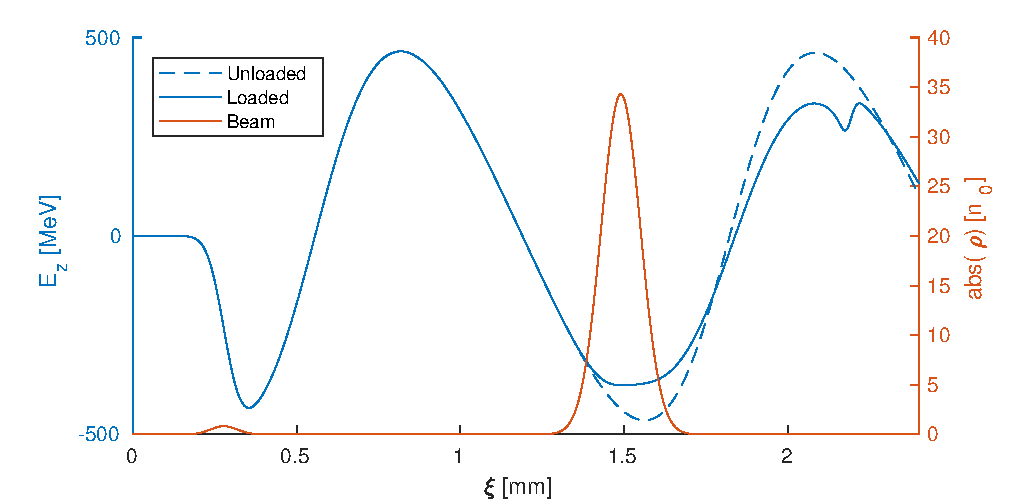
\includegraphics[width=\linewidth,trim={2mm 0mm 2mm 0mm},clip]{figures/beamLoading}
    \caption{\label{Fig:BeamLoading} The top plot compares the unloaded longitudinal e-field (no witness beam, blue.
        dashed  line) and the loaded e-field (blue line) along the beam axis. The magnitude of the beam density along
        the axis is shown (red line) for reference. The bottom plot compares the plasma density along the beam axis for
        a drive beam with no witness beam (dashed green line), witness beam with no drive beam (dash-dotted green line),
        and both witness and drive beam present (continuous green line). $\xi = z - tc$ is the position in the
        simulation box and both beams travel towards the left. The beam and plasma densities arein units of initial
        plasma density $n_{0} = 7\nexp{-14}\unit{cm}^{-3}$.}
\end{figure}

\begin{figure}[hbt]
    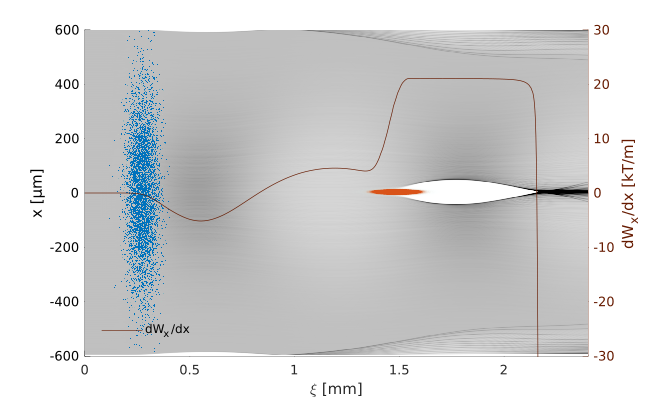
\includegraphics[width=\linewidth,trim={2mm 0mm 2mm 0mm},clip]{figures/plasmaDenTWake}
    \caption{\label{Fig:PlasmaDenTWake} The plasma density in grey with the proton beam (blue) and the electron beam
        (red) superimposed. The line plot indicates the transverse wakefield gradient $dW_{x}/dx$ where
        $W_{x} = E_{x} - v_{b} B_{y}$, evaluated along the beam axis.}
\end{figure}

%~ - describe proton beam wake structure [similar to that of a modulated proton beam] (simulation results to show:
%~   unloaded wake)

The single drive beam setup is designed to behave similarly to the self-modulated case. However, since the drive beam is
prevented from significant transverse evolution, we are presented with an idealised case where the electron witness beam
sees consistent fields throughout the plasma stage. The field generated by the proton drive bunch is seen as the dotted
line in figure \ref{Fig:BeamLoading}. With a proton beam density $n_{pb} \simeq n_{0}$, we are in the quasi-linear
regime but near non-linear \cite{rosenzweig:2010}. There is some depletion of plasma electrons, but not enough to form a
bubble. The dashed green line in the lower part of figure \ref{Fig:BeamLoading} shows that the on-axis plasma density
has a depletion of $67\%$.

%~ - by varying the current of the electron beam, the electron beam may load the wake and the longitudinal field can be
%~   flatten and energy spread reduced [well known result, Tzoufras]

The witness bunch generates its own wakefield, which in the accelerating phase cancels out the $E_{z}$ field generated
by the drive bunch. For a finite length bunch this causes the particles in the tail of the witness bunch to be
accelerated less than those at the front resulting in high energy spread in exchange for high energy transfer
\cite{van_der_meer:1985}. Since $E_{z} \propto \rho_{b}$, a beam profile $\rho_{b}(\xi)$ that perfectly flattens the
accelerating field within the witness beam, reduces energy spread to zero. The ideal shape is triangular or trapezoidal
with the peak density in the direction of the beam velocity \cite{katsouleas:1987, tzoufras:2009}.

%~ - the electron beam blows out the remaining plasma electrons. The transverse fields are dominated by the linear
%~   focusing fields originating from the ion background, leading to emittance preservation of the part of the electron
%~   beam inside the bubble [loading of a quasi-linear wake, and still get emittance preservation: this is new]
%~   (simulation results to show: loaded wake, with bubble - many different aspects of this, trans., long. field,
%~   electron densities etc. )

For Gaussian beams a reasonable flat field and consequently low energy spread can be achieved by controlling the charge
density. In our case, with a matched beam to the plasma density \ref{EQ:Matched}, we are limited on how much total
charge we can accelerate. The test case shown in figures \ref{Fig:BeamLoading} and \ref{Fig:PlasmaDenTWake} has a total
charge of $100\unit{pC}$ with a $\sigma_{r}=5.23\unit{\mu m}$ matching an initial normalised emittance
$\epsilon_{0} = 2\unit{\mu m}$.

\begin{figure}[hbt]
    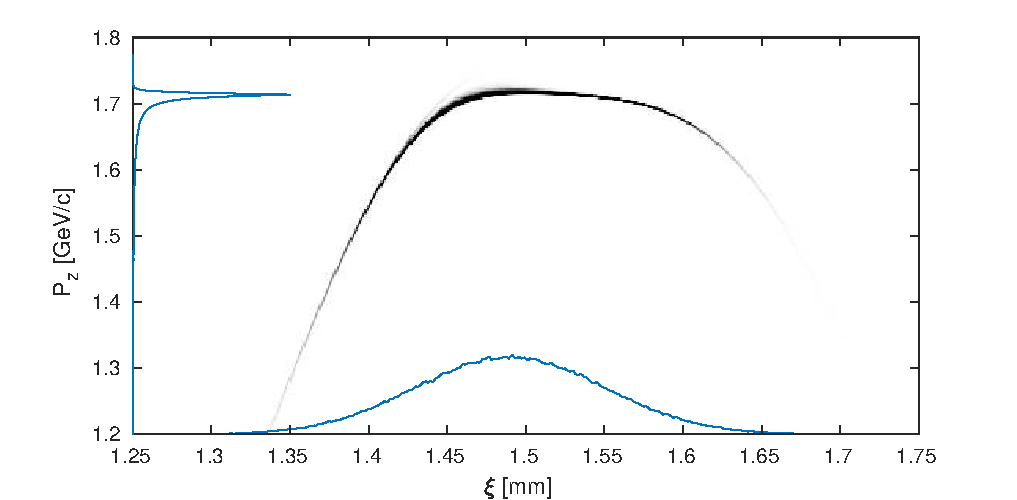
\includegraphics[width=\linewidth,trim={2mm 0mm 2mm 0mm},clip]{figures/beamPhaseSpace}
    \caption{\label{Fig:BeamPS} Phase space charge distribution of a $100\unit{pC}$, $60\unit{\mu m}$ long witness beam
        after $4\unit{m}$ of plasma. Mean momentum is $1.67\unit{GeV/c}$ with an RMS spread of $87\unit{MeV/c}$
        ($5.2\%$) for the full beam.}
\end{figure}

As illustrated in figure \ref{Fig:BeamPS}, our base case of a $100\unit{pC}$, $60\unit{\mu m}$ long witness beam indeed
shows a difference in energy transfer to the tail of the beam. Also the front of the beam has a large tail in momentum
space. The positioning of the witness beam is chosen to put the bulk of the charge as close to the peak accelerating
field as possible, as can be seen in figure \ref{Fig:BeamLoading}.

Due to the high charge density resulting from a very narrow beam, the witness beam's own wakefield reaches the full
non-linear regime with $n_{eb} \approx 35\times n_{0}$. The plasma region reaches full depletion close to the peak of
the electron beam, which in turn generates strong focusing fields, with gradients of $20\unit{kT/m}$ near the beam axis
(see figure \ref{Fig:PlasmaDenTWake}).

%~ - the acceleration and the transverse emittance stable on long timescales (simulation results to show: transverse and
%~   longitudinal phase spaces, space long simulation)



%~ - in this regime, emittance preservation is robustness to drive-witness offset [this is new] (simulation results to
%~   show: transverse and longitudinal phase spaces, long offset simulation)

% ******************************************************************************************************************** %
\section[\label{S:PO}]{Parameter Optimisation}
%~ Sec N+1: Parameter optimization, or, parameter scaling [in this section we describe how to optimize the electron
%~ beam, and preferably some scalings]
%~ - how to select electron beam parameters:
%~ - longitudinal parameters bunch length and current (simulations results to show: overloaded/underloaded cases)
%~ - transverse parameters of electron emittance / matching [too large, outside bubble.  Do we see increased head
%~   erosion -> faster decay]?  (simulations results to show: evolution of high emittance vs low emittance cases)
%~ (- plasma density?)
% ******************************************************************************************************************** %


% ******************************************************************************************************************** %
\section[\label{S:D}]{Discussion}
% ******************************************************************************************************************** %

% ******************************************************************************************************************** %
\section[\label{S:C}]{Conclusion}
% discussion of optimal electron beam parameters
% implications for AWAKE Run 2
% ******************************************************************************************************************** %

\section[\label{Ack}]{Acknowledgements}
% ******************************************************************************************************************** %

The simulations forming the basis for this study have been made possible using the open source version of QuickPIC
released in early 2017 and owned by UCLA.

These numerical simulations have been made possible through access to the Abel computing cluster in Oslo, Norway
maintained by UNINETT Sigma2 AS and financed by the Research Council of Norway, the University of Bergen, the University
of Oslo, the University of Tromsø and the Norwegian University of Science and Technology. Project code: nn9303k.

The authors would also like to acknowledge the OSIRIS Consortium for providing access to the OSIRIS framework. OSIRIS
was used extensively for simulations leading up to the work presented in this paper.

% ******************************************************************************************************************** %
\bibliography{Bibliography}
\end{document}
% ******************************************************************************************************************** %
